\documentclass[../main.tex]{subfiles}
\begin{document}
\chapter{Implementazione dei controlli di sicurezza FedRAMP in Moon Cloud}
%\addcontentsline{toc}{chapter}{Introduzione}
%\chaptermark{Introduzione}
\section{Introduzione}
In questo capitolo verrà effettuata un'analisi dei controlli di sicurezza elencati nel capitolo precedente, classificandoli in \textit{controlli automatici} e \textit{controlli procedurali}. Dopodiché verra offerta una possibile implementazione per ciascuna delle due tipologie di controlli, i quali verranno integrati in Moon Cloud. Per i controlli automatici sarà utilizzato Open Scap, uno strumento per il l'auditing realizzato da Red Hat e certificato dal NIST. I controlli procedurali invece, eseguono l'\textit{processi di business} e vanno ad indirizzare tutte quelle proprietà di carattere puramente qualitativo per cui è fondamentale l'interazione umana.
Questi saranno implementati con un \textit{driver Moon Cloud ad interazione umana}, che somministra un questionario online ad un target.

\section{Analisi dei controlli di sicurezza}
Verranno ora proposte alcune tabelle di riepilogo dei controlli di sicurezza di FedRAMP, suddivisi per famiglia, dei quali viene indicata la \textit{baseline} di riferimento e la tipologia (\textit{A}, automatizzabile / \textit{P} procedurale (interazione umana) / \textit{A/P} composizione di approccio automatico e manuale).

I controlli di sicurezza, essendo proposti in modo astratto così da poter coprire il più vasto numero di scenari, vanno poi comunque studiati e implementati sulla base delle caratteristiche e del contesto del sistema target.
\subsection{Access Control}
%\makeatletter
\begin{ltabulary}{|p{2cm}|p{8cm}|L|p{1cm}|}
  \toprule
    \hline
    \textbf{ID}    & \textbf{Nome}                                                        & \textbf{Baseline} & \textbf{Tipo} \\ \hline
  \midrule
  \endhead
  \textbf{AC-1 }   & access control policy and procedures                                 & Basso             & P             \\ \hline
  \textbf{AC-2 }   & account management                                                   & Basso             & A/P           \\ \hline
AC-2 (1)           & automated system account management                                  & Moderato          & A/P           \\ \hline
AC-2 (2)           & removal of temporary / emergency accounts                            & Moderato          & A             \\ \hline
AC-2 (3)           & disable inactive accounts                                            & Moderato          & A/P           \\ \hline
AC-2 (4)           & automated audit actions                                              & Moderato          & A             \\ \hline
AC-2 (5)           & inactivity logout                                                    & Moderato          & A             \\ \hline
AC-2 (7)           & role-based schemes                                                   & Moderato          & P             \\ \hline
AC-2 (9)           & restrictions on use of shared groups / accounts                      & Moderato          & A             \\ \hline
AC-2 (10)          & shared / group account credential termination                        & Moderato          & A/P           \\ \hline
AC-2 (12)          & account monitoring / atypical usage                                  & Moderato          & P             \\ \hline
\textbf{AC-3 }     & access enforcement                                                   & Basso             & A/P           \\ \hline
\textbf{AC-4 }     & information flow enforcement                                         & Moderato          & A/P           \\ \hline
AC-4 (21)          & physical / logical separation of information flows                   & Moderato          & A/P           \\ \hline
\textbf{AC-5 }     & separation of duties                                                 & Moderato          & A/P           \\ \hline
\textbf{AC-6 }     & least privilege                                                      & Moderato          & A/P           \\ \hline
AC-6 (1)           & authorize access to security functions                               & Moderato          & A             \\ \hline
AC-6 (2)           & non-privileged access for nonsecurity functions                      & Moderato          & A             \\ \hline
AC-6 (5)           & privileged accounts                                                  & Moderato          & A             \\ \hline
AC-6 (9)           & auditing use of privileged functions                                 & Moderato          & A             \\ \hline
AC-6 (10)          & prohibit non-privileged users from execution of privileged functions & Moderato          & A             \\ \hline
\textbf{AC-7 }     & unsuccessful logon attempts                                          & Basso             & A             \\ \hline
\textbf{AC-8 }     & system use notification                                              & Basso             & A             \\ \hline
\textbf{AC-10}     & concurrent session control                                           & Moderato          & A             \\ \hline
\textbf{AC-11}     & session lock                                                         & Moderato          & A             \\ \hline
AC-11 (1)          & pattern-hiding displays                                              & Moderato          & A             \\ \hline
\textbf{AC-12}     & session termination                                                  & Moderato          & A             \\ \hline
\textbf{AC-14}     & "permitted actions without identification or authentication"         & Basso             & A/P           \\ \hline
\textbf{AC-17}     & remote access                                                        & Basso             & A/P           \\ \hline
AC-17 (1)          & automated monitoring / control                                       & Moderato          & P             \\ \hline
AC-17 (2)          & protection of confidentiality / integrity using encryption           & Moderato          & A/P           \\ \hline
AC-17 (3)          & managed access control points                                        & Moderato          & A             \\ \hline
AC-17 (4)          & privileged commands / access                                         & Moderato          & A/P \ \hline
AC-17 (9)          & disconnect / disable access                                          & Moderato          & A/P           \\ \hline
\textbf{AC-18}     & wireless access                                                      & Basso             & A/P           \\ \hline
AC-18 (1)          & authentication and encryption                                        & Moderato          & A/P           \\ \hline
\textbf{AC-19}     & access control for mobile devices                                    & Basso             & A             \\ \hline
AC-19 (5)          & full device / container-based encryption                             & Moderato          & A             \\ \hline
\textbf{AC-20}     & use of external information systems                                  & Basso             & A             \\ \hline
AC-20 (1)          & limits on authorized use                                             & Moderato          & A             \\ \hline
AC-20 (2)          & portable storage devices                                             & Moderato          & A             \\ \hline
\textbf{AC-21}     & information sharing                                                  & Moderato          & P             \\ \hline
    \textbf{AC-22} & publicly accessible content                                          & Basso             & A/P           \\ \hline
\end{ltabulary}
%AC17 1
%\makeatother

Il principio seguito è il \textit{least-privilege}, che consiste nel concedere a ciascun utente i privilegi minimi di accesso necessari esclusivamente al compimento delle azioni di suo interesse.
Abbiamo un totale di 43 controlli, di cui 22 sono completamente automatizzabili, 5 sono di carattere procedurale e necessitano interazione umana, mentre per 16 di questi è necessario adottare un approccio ibrido.
Pertanto possiamo utilizzare un approccio totalmente automatico solo nel 51.1\%  dei casi, tuttavia considerando anche i casi in cui è richiesta sia la modalità automatica che quella manuale, la percentuale sale all'88\%.
Bisogna però notare che nel caso sia utilizzato Moon Cloud per monitorare i processi di autenticazione e autorizzazione, i controlli AC-6 (9) e AC-17 (1) possono essere automaticamente soddisfatti.


\subsection{Awareness \& training}
\makeatletter

\begin{ltabulary}{|p{2cm}|p{8cm}|L|p{1cm}|}
    \hline
    \textbf{ID}     &\textbf{Nome}                                                          & \textbf{Baseline} & \textbf{Tipo}  \\    \hline
  \endhead

    \textbf{AT-1}     & security awareness and training policy and procedures                  & Basso & P \\ \hline
    \textbf{AT-2}     & security awareness training                                           & Basso & P \\ \hline
    AT-2 (2)          & insider threat                                                        & Moderato & P \\ \hline
    \textbf{AT-3}     & role-based security training                                          & Basso & P \\ \hline
    \textbf{AT-4}     & security training records                                             & Basso & P \\ \hline
\end{ltabulary}
\begin{center}
\captionof{table}{Controlli della classe AT} 
\end{center}
\makeatother
I controlli della famiglia \textit{awareness and training} sono soltanto 5, e per ciascuno di essi è richiesta intrinsecamente l'interazione umana.
Questa, infatti, misura il grado di consapevolezza dell'utente rispetto alle politiche e alle procedure di sicurezza. 

L'approccio ibrido può essere utilizzato qualora si voglia adottare un sistema automatico per la valutazione delle conoscenze dell'utente oppure l'individuazione di minacce provenienti dall'esterno.


\subsection{Audit and accountability}
\makeatletter

\begin{ltabulary}{|p{2cm}|p{8cm}|L|p{1cm}|}
    \hline
    \textbf{ID}     &\textbf{Nome}                                                          & \textbf{Baseline} & \textbf{Tipo}  \\    \hline
  \endhead

  \textbf{AU-1 }		&			"audit and accountability policy and procedures" 		        &						 Basso 		&						 P \\ \hline
  \textbf{AU-2 }		&			 audit events 		                                            &						 Basso 		&						 P\\ \hline
AU-2 (3) 	&			 reviews and updates 		                                    &						 Medio 		&						 P \\ \hline
\textbf{AU-3 }		&			 content of audit records 		                                &						 Basso 		&						 A \\ \hline
AU-3 (1) 	&			 additional audit information                   	        	&						 Medio 		&						 P \\ \hline
\textbf{AU-4 }		&			 audit storage capacity 	                                	&						 Basso 		&						 A \\ \hline
\textbf{AU-5 }		&			 response to audit processing failures 	                    	&						 Basso 		&						 A \\ \hline
\textbf{AU-6 }		&			 "audit review, analysis, and reporting" 	                	&						 Basso 		&						 P \\ \hline
AU-6 (1) 	&			 "process integration"                                      	&						 Medio 		&						 P \\ \hline
AU-6 (3) 	&			 "correlate audit repositories"                         		&						 Medio 		&						 P \\ \hline
\textbf{AU-7 }		&			 audit reduction and report generation 	                    	&						 Medio 		&						 A \\ \hline
AU-7 (1) 	&			 automatic processing                                   		&						 Medio 		&						 A \\ \hline
\textbf{AU-8 }		&			 time stamps                                            		&						 Basso 		&						 A \\ \hline
AU-8 (1) 	&			 synchronization with authoritative time source         		&						 Medio 		&						 A \\ \hline
\textbf{AU-9 }		&			 protection of audit information                        		&						 Basso 		&						 A \\ \hline
AU-9 (2) 	&			 audit backup on separate physical systems / components 		&						 Medio 		&						 A \\ \hline
AU-9 (4) 	&			 access by subset of privileged users 	                    	&						 Medio 		&						 A/P \\ \hline
\textbf{AU-11} 		&			 audit record retention                                 		&						 Basso 		&						 A \\ \hline
\textbf{AU-12} 		&			 audit generation 	                                        	&						 Basso 		&						 A \\ \hline
\end{ltabulary}
\makeatother
Dei 19 controlli sull'\textit{auditing}, 11 possono essere effettuati in maniera completamente automatica, 1 richiede un approccio ibrido e 7 richiedono l'interazione umana.
Per cui si può affermare che nel 63\% dei casi, è adottabile un approccio automatico.

%implementazione -> controllo openstack ntp che si mappa su timestamps di AU 8, + auditctl correttamente configurato + questione delle partizioni



\subsection{Certification, Accreditation \& Security Assessment}
\makeatletter

\begin{ltabulary}{|p{2cm}|p{8cm}|L|p{1cm}|}
    \hline
    \textbf{ID}     &\textbf{Nome}                                                          & \textbf{Baseline} & \textbf{Tipo}  \\    \hline
  \endhead


\textbf{CA-1} 		& "security assessment and authorization policy and procedures" 		& Basso 		& P \\ \hline
\textbf{CA-2} 		& security assessments 	                                            	& Basso 		& P \\ \hline
CA-2 (1) 	        & independent assessors                                            		& Basso 		& P \\ \hline
CA-2 (2) 	        & specialized assessments 	                                        	& Moderato 		& P \\ \hline
CA-2 (3) 	        & external organizations 	                                        	& Moderato 		& P \\ \hline
\textbf{CA-3} 		& system interconnections 	                                        	& Basso 		& P \\ \hline
CA-3 (3) 	        & unclassified non-national security system connections 	           	& Moderato 		& P \\ \hline
CA-3 (5) 	        & restrictions on external system connections                   		& Moderato 		& P \\ \hline
\textbf{CA-5} 		& plan of action and milestones                                    		& Basso 		& P \\ \hline
\textbf{CA-6} 		& security authorization                                        		& Basso 		& P \\ \hline
\textbf{CA-7} 		& continuous monitoring                                         		& Basso 		& P \\ \hline
CA-7 (1) 	        & independent assessment                                        		& Moderato 		& P \\ \hline
\textbf{CA-8} 		& penetration testing 	                                            	& Moderato 		& P \\ \hline
CA-8 (1) 	        & independent penetration agent or team 	                           	& Moderato 		& P \\ \hline
\textbf{CA-9} 		& internal system connections                                   		& Basso 		& P \\ \hline
\end{ltabulary}
\begin{center}
\captionof{table}{Controlli della classe CA} 
\end{center}
\makeatother

I controlli di questa classe sono tutti di tipo procedurale, e non possono essere automatizzati: si tratta infatti di una serie di dichiarazioni che il responsabile della sicurezza IT del provider deve compilare.


\subsection{Configuration Management}
\makeatletter

\begin{ltabulary}{|p{2cm}|p{8cm}|L|p{1cm}|}
    \hline
    \textbf{ID}     &\textbf{Nome}                                                          & \textbf{Baseline} & \textbf{Tipo}  \\    \hline
  \endhead


CM-1      & "configuration management policy and procedures"                             & Basso    & P   \\ \hline
CM-2      & baseline configuration                                                       & Basso    & P   \\ \hline
CM-2 (1)  & previews and updates                                                          & Moderato & P   \\ \hline
CM-2 (2)  & automation support for accuracy / currency                                   & Moderato & P   \\ \hline
CM-2 (3)  & retention of previous configurations                                         & Moderato & P   \\ \hline
CM-2 (7)  & configure systems, components, or devices for high-risk areas                & Moderato & P   \\ \hline
CM-3      & configuration change control                                                 & Moderato & P   \\ \hline
CM-4      & security impact analysis                                                     & Basso    & P   \\ \hline
CM-5      & access restrictions for change                                               & Moderato & A/P \\ \hline
CM-5 (1)  & automated access enforcement / auditing                                      & Moderato & A   \\ \hline
CM-5 (3)  & signed components                                                            & Moderato & A   \\ \hline
CM-5 (5)  & "access restrictions for change | limit production / operational privileges" & Moderato & A   \\ \hline
CM-6      & configuration settings                                                       & Basso    & A/P \\ \hline
CM-6 (1)  & automated central management / application / verification                    & Moderato & P   \\ \hline
CM-7      & least functionality                                                          & Basso    & A/P \\ \hline
CM-7 (1)  & periodic review                                                              & Moderato & P   \\ \hline
CM-7 (2)  & prevent program execution                                                    & Moderato & A   \\ \hline
CM-7 (5)  & authorized software / whitelisting                                           & Moderato & A   \\ \hline
CM-8      & information system component inventory                                       & Basso    & A/P \\ \hline
CM-8 (1)  & updates during installations / removals                                      & Moderato & A/P \\ \hline
CM-8 (3)  & automated unauthorized component detection                                   & Moderato & A   \\ \hline
CM-8 (5)  & no duplicate accounting of components                                        & Moderato & A   \\ \hline
CM-9      & configuration management plan                                                & Moderato & P   \\ \hline
CM-10     & software usage restrictions                                                  & Basso    & A/P \\ \hline
CM-10 (1) & open source software                                                         & Moderato & P   \\ \hline
CM-11     & user-installed software                                                      & Basso    & A/P \\ \hline
\end{ltabulary}
\begin{center}
\captionof{table}{Controlli della classe CM} 
\end{center}

I controlli appartenenti a questa famiglia rientrano nella tipologia "controllo operativo". Molti di questi sono quindi controlli essenzialmente procedurali, in quanto consistono nel verificare l'esistenza e la conformità delle policy per la gestione dei cambiamenti.
Gran parte delle conseguenze di queste policy, però, contengono elementi di carattere tecnico; per questa ragione, in alcuni casi, l'esecuzione degli stessi può avvenire in modo automatico o semi-automatico.
In particolare i meccanismi automatici possono essere utilizzati in 14 casi su 26, garantendo quindi una copertura del 53\%. Di questi 14 controlli effettuabili in maniera automatica, la metà devono però essere eseguiti con un approccio ibrido.
\makeatother


\subsection{Contingency Planning}
\makeatletter

\begin{ltabulary}{|p{2cm}|p{8cm}|L|p{1cm}|}
    \hline
    \textbf{ID}     &\textbf{Nome}                                                          & \textbf{Baseline} & \textbf{Tipo}  \\    \hline
  \endhead


  \textbf{CP-1 } & "contingency planning policy and procedures"   & Basso    & P   \\ \hline
  \textbf{CP-2 } & contingency plan                               & Basso    & P   \\ \hline
CP-2 (1)         & coordinate with related plans                  & Moderato & P   \\ \hline
CP-2 (2)         & capacity planning                              & Moderato & P   \\ \hline
CP-2 (3)         & resume essential missions / business functions & Moderato & P   \\ \hline
CP-2 (8)         & identify critical assets                       & Moderato & P   \\ \hline
\textbf{CP-3 }   & contingency training                           & Basso    & P   \\ \hline
\textbf{CP-4 }   & contingency plan testing                       & Basso    & P   \\ \hline
CP-4 (1)         & coordinate with related plans                  & Moderato & P   \\ \hline
\textbf{CP-6 }   & alternate storage site                         & Moderato & A/P \\ \hline
CP-6 (1)         & separation from primary site                   & Moderato & P   \\ \hline
CP-6 (3)         & accessibility                                  & Moderato & P   \\ \hline
\textbf{CP-7 }   & alternate processing site                      & Moderato & P   \\ \hline
CP-7 (1)         & separation from primary site                   & Moderato & P   \\ \hline
CP-7 (2)         & accessibility                                  & Moderato & P   \\ \hline
CP-7 (3)         & priority of service                            & Moderato & P   \\ \hline
\textbf{CP-8 }   & telecommunications services                    & Moderato & P   \\ \hline
CP-8 (1)         & priority of service provisions                 & Moderato & P   \\ \hline
CP-8 (2)         & single points of failure                       & Moderato & P   \\ \hline
\textbf{CP-9 }   & information system backup                      & Basso    & A/P \\ \hline
CP-9 (1)         & testing for reliability / integrity            & Moderato & A   \\ \hline
CP-9 (3)         & separate storage for critical information      & Moderato & A/P \\ \hline
\textbf{CP-10}   & information system recovery and reconstitution & Basso    & P   \\ \hline
CP-10 (2)        & transaction recovery                           & Moderato & A/P \\ \hline
\end{ltabulary}
\captionof{table}{Controlli della classe CP} 

La realizzazione del piano di contingenza è di carattere prettamente procedurale per definizione; l'obiettivo è infatti quello di studiare gli impatti sul business di possibili incidenti informatici, pianificare le operazioni di \textit{incident response}, un piano per il recupero dall'incidente (\textit{disastery recovery}) e le eventuali misure prese per garantire la \textit{business continuity}.


Proprio le ultime citate sono l'oggetto dei pochi controlli parzialmente automatizzabili: nel caso del \textit{CP-6}, ad esempio, che prevede l'esistenza di una locazione alternativa per lo \textit{storage} dei dati, si può verificare che entrambe le locazioni siano sempre sincronizzate e che le proprietà di confidenzialità e integrità nella ridondanza geografica siano rispettate.


La stessa considerazione può essere fatta per i sistemi di backup dei dati (CP-9) e dei log delle transazioni (CP-10), tenendo anche conto del fatto che le informazioni critiche devono essere trattate separatamente (CP-9 (3)). Eventuali sistemi automatici possono essere utilizzati anche per la verifica dell'affidabilità, l'integrità, il testing (e la effettiva possibilità di recupero dati).

L'approccio automatico può essere usato nel 16\% dei casi.
\makeatother


\subsection{Identification and Authentication}
\makeatletter

\begin{ltabulary}{|p{2cm}|p{8cm}|L|p{1cm}|}
    \hline
    \textbf{ID}     &\textbf{Nome}                                                          & \textbf{Baseline} & \textbf{Tipo}  \\    \hline
  \endhead

\textbf{IA-1} & "identification and authentication policy and procedures"                         & Basso    & P   \\ \hline
\textbf{IA-2} & "identification and authentication (organizational users)"                        & Basso    & P   \\ \hline
IA-2 (1)      & network access to privileged accounts                                             & Basso    & A   \\ \hline
IA-2 (2)      & network access to non-privileged accounts                                         & Moderato & A   \\ \hline
IA-2 (3)      & local access to privileged accounts                                               & Moderato & A   \\ \hline
IA-2 (5)      & "identification and authentication (organizational users) | group authentication" & Moderato & A   \\ \hline
IA-2 (8)      & network access to privileged accounts - replay resistant                          & Moderato & A   \\ \hline
IA-2 (11)     & remote access - separate device                                                   & Moderato & A   \\ \hline
IA-2 (12)     & acceptance of piv credentials                                                     & Basso    & A   \\ \hline
\textbf{IA-3} & device identification and authentication                                          & Moderato & A   \\ \hline
\textbf{IA-4} & identifier management                                                             & Basso    & P   \\ \hline
IA-4 (4)      & identify user status                                                              & Moderato & P   \\ \hline
\textbf{IA-5} & authenticator management                                                          & Basso    & A/P \\ \hline
IA-5 (1)      & password-based authentication                                                     & Basso    & A   \\ \hline
IA-5 (2)      & pki-based authentication                                                          & Moderato & A   \\ \hline
IA-5 (3)      & in-person or trusted third-party registration                                     & Moderato & A   \\ \hline
IA-5 (4)      & automated support for password strength determination                             & Moderato & A   \\ \hline
IA-5 (6)      & protection of authenticators                                                      & Moderato & A   \\ \hline
IA-5 (7)      & no embedded unencrypted static authenticators                                     & Moderato & A   \\ \hline
IA-5 (11)     & hardware token-based authentication                                               & Basso    & A   \\ \hline
\textbf{IA-6} & authenticator feedback                                                            & Basso    & A   \\ \hline
\textbf{IA-7} & cryptographic module authentication                                               & Basso    & A   \\ \hline
\textbf{IA-8} & identification and authentication (non- organizational users)                     & Basso    & A   \\ \hline
IA-8 (1)      & acceptance of piv credentials from other agencies                                 & Basso    & A   \\ \hline
IA-8 (2)      & acceptance of third-party credentials                                             & Basso    & A   \\ \hline
IA-8 (3)      & use of ficam-approved products                                                    & Basso    & A   \\ \hline
IA-8 (4)      & use of ficam-issued profiles                                                      & Basso    & A   \\ \hline
\end{ltabulary}
\begin{center}
\captionof{table}{Controlli della classe IA} 
\end{center}

I controlli della famiglia di \textit{identificazione e autenticazione} sono perlopiù di carattere tecnico e pertanto in gran parte automatizzabili (nell'85\% dei casi).
Questi hanno una stretta correlazione con i controlli della famiglia \textit{controllo degli accessi} e di \textit{auditing}, già trattate, e manifestano la necessità per il provider di mantenere \textit{accountability} e \textit{non-repudiation}. Pertanto si tratta di controlli effettuati sulla resistenza delle credenziali agli attacchi, sulla sicurezza del processo di autenticazione e sulla possibilità di ricondurre con esattezza tutte le operazioni svolte sul sistema all'attore che le ha compiute, sia esso un servizio automatico o un utente umano.
Molti di questi, tuttavia, sono anche di carattere ibrido o procedurale, poiché basati sulle dichiarazioni del provider stesso.

\makeatother


\subsection{Incident response}
\begin{ltabulary}{|p{2cm}|p{8cm}|L|p{1cm}|}
    \hline
    \textbf{ID}     &\textbf{Nome}                                                          & \textbf{Baseline} & \textbf{Tipo}  \\    \hline
  \endhead

\textbf{IR-1} & incident response policy and procedures                      & Basso    & P \\ \hline
\textbf{IR-2} & incident response training                                   & Basso    & P \\ \hline
\textbf{IR-3} & incident response testing                                    & Moderato & P \\ \hline
IR-3 (2)      & coordination with related plans                              & Moderato & P \\ \hline
\textbf{IR-4} & incident handling                                            & Basso    & P \\ \hline
IR-4 (1)      & automated incident handling processes                        & Moderato & P \\ \hline
\textbf{IR-5} & incident monitoring                                          & Basso    & P \\ \hline
\textbf{IR-6} & incident reporting                                           & Basso    & P \\ \hline
IR-6 (1)      & automated reporting                                          & Moderato & P \\ \hline
\textbf{IR-7} & incident response assistance                                 & Basso    & P \\ \hline
IR-7 (1)      & automation support for availability of information / support & Moderato & P \\ \hline
IR-7 (2)      & coordination with external providers                         & Moderato & P \\ \hline
\textbf{IR-8} & incident response plan                                       & Basso    & P \\ \hline
\textbf{IR-9} & information spillage response                                & Moderato & P \\ \hline
IR-9 (1)      & responsible personnel                                        & Moderato & P \\ \hline
IR-9 (2)      & training                                                     & Moderato & P \\ \hline
IR-9 (3)      & post-spill operations                                        & Moderato & P \\ \hline
IR-9 (4)      & exposure to unauthorized personnel                           & Moderato & P \\ \hline
\end{ltabulary}
\begin{center}
\captionof{table}{Controlli della classe IR} 
\end{center}

Nel caso dell'\textit{incident response}, le attività sono essenzialmente procedurali, per definizione.
La componente automatica può essere aggiunta in alcuni casi come misura complementare, ad esempio nel caso di \textit{IR-4} (meccanismi di gestione degli incidenti automatici), \textit{IR-5} (esistenza di meccanismi efficaci per il monitoraggio degli incidenti), \textit{IR-6} (meccanismi di reporting automatico) e \textit{IR-9} (fuoriuscita di informazioni per esposizione delle stesse a personale non autorizzato). 
Per soddisfare \textit{IR-4}, ad esempio, si può controllare la presenza e la corretta configurazione di meccanismi di protezione istantanei (ad esempio reazioni automatiche del firewall in relazione ad eventuali pattern di attacco)
Nel caso di \textit{IR-5} possono essere effettuate misurazioni sulla presenza e la corretta configurazione di meccanismi IDS e IPS, unitamente alla frequenza degli aggiornamenti delle definizioni.
\vfill
\newpage


\subsection{Maintenance}
\makeatletter

\begin{ltabulary}{|p{2cm}|p{8cm}|L|p{1cm}|}
    \hline
    \textbf{ID} & \textbf{Nome}                            & \textbf{Baseline} & \textbf{Tipo} \\ \hline
  \endhead
\textbf{MA-1}   & system maintenance policy and procedures & Basso             & P             \\ \hline
\textbf{MA-2}   & controlled maintenance                   & Basso             & P             \\ \hline
\textbf{MA-3}   & maintenance tools                        & Moderato          & A/P           \\ \hline
MA-3 (1)        & inspect tools                            & Moderato          & A             \\ \hline
MA-3 (2)        & inspect media                            & Moderato          & A             \\ \hline
MA-3 (3)        & prevent unauthorized removal             & Moderato          & A             \\ \hline
\textbf{MA-4}   & nonlocal maintenance                     & Basso             & P             \\ \hline
MA-4 (2)        & document nonlocal maintenance            & Moderato          & P             \\ \hline
\textbf{MA-5}   & maintenance personnel                    & Basso             & P             \\ \hline
MA-5 (1)        & individuals without appropriate access   & Moderato          & P             \\ \hline
\textbf{MA-6}   & timely maintenance                       & Moderato          & A/P           \\ \hline
\end{ltabulary}

Anche in questo caso ci troviamo in presenza di controlli di carattere perlopiù procedurale, nonostante l'approccio automatico possa essere utilizzato per garantire la correttezza delle operazioni svolte (ad esempio in \textit{MA-3(1)}, \textit{MA-3(2)} e \textit{MA-3(3)})

\makeatother


\subsection{Media protection}
\begin{ltabulary}{|p{2cm}|p{8cm}|L|p{1cm}|}
    \hline
    \textbf{ID}     &\textbf{Nome}                                                          & \textbf{Baseline} & \textbf{Tipo}  \\    \hline
  \endhead
\textbf{MP-1} & media protection policy and procedures & Basso    & P \\ \hline
\textbf{MP-2} & media access                           & Basso    & P \\ \hline
\textbf{MP-3} & media marking                          & Moderato & P \\ \hline
\textbf{MP-4} & media storage                          & Moderato & P \\ \hline
\textbf{MP-5} & media transport                        & Moderato & A/P \\ \hline
MP-5 (4)      & cryptographic protection               & Moderato & A/P \\ \hline
\textbf{MP-6} & media sanitization                     & Basso    & P \\ \hline
MP-6 (2)      & equipment testing                      & Moderato & P \\ \hline
\textbf{MP-7} & media use                              & Basso    & A/P \\ \hline
MP-7 (1)      & prohibit use without owner             & Moderato & A/P \\ \hline
\end{ltabulary}
\captionof{table}{Controlli della classe MP} 
Questa categoria di controlli riguarda perlopiù processi di business nei quali è implicato l'utilizzo di dispositivi multimediali per il trasferimento delle informazioni. Si tratta perciò di controlli che devono essere verificati con interazione umana, anche se possono essere effettuate alcune verifiche in modo automatico, come nel caso della proprietà \textit{MP-5} che verifica l'utilizzo della crittografia nel trasporto dei dati effettuato con dispositivi multimediali (CD, DVD, Pendrive).



\subsection{Physical and environmental protection}
\makeatletter

\begin{ltabulary}{|p{2cm}|p{8cm}|L|p{1cm}|}
    \hline
    \textbf{ID} & \textbf{Nome}                                                 & \textbf{Baseline} & \textbf{Tipo} \\ \hline
  \endhead
\textbf{PE-1 }  & "physical and environmental protection policy and procedures" & Basso             & A/P           \\ \hline
\textbf{PE-2 }  & physical access authorizations                                & Basso             & P             \\ \hline
\textbf{PE-3 }  & physical access control                                       & Basso             & A/P           \\ \hline
\textbf{PE-4 }  & access control for transmission medium                        & Moderato          & A/P           \\ \hline
\textbf{PE-5 }  & access control for output devices                             & Moderato          & A/P           \\ \hline
\textbf{PE-6 }  & monitoring physical access                                    & Basso             & A/P           \\ \hline
PE-6 (1)        & intrusion alarms / surveillance equipment                     & Moderato          & A/P           \\ \hline
\textbf{PE-8 }  & visitor access records                                        & Basso             & A/P           \\ \hline
\textbf{PE-9 }  & power equipment and cabling                                   & Moderato          & A/P           \\ \hline
\textbf{PE-10}  & emergency shutoff                                             & Moderato          & A/P           \\ \hline
\textbf{PE-11}  & emergency power                                               & Moderato          & A/P           \\ \hline
\textbf{PE-12}  & emergency lighting                                            & Basso             & A/P           \\ \hline
\textbf{PE-13}  & fire protection                                               & Basso             & A/P           \\ \hline
PE-13 (2)       & suppression devices / systems                                 & Moderato          & A/P           \\ \hline
PE-13 (3)       & automatic fire suppression                                    & Moderato          & A/P           \\ \hline
\textbf{PE-14}  & temperature and humidity controls                             & Basso             & A/P           \\ \hline
PE-14 (2)       & monitoring with alarms / notifications                        & Moderato          & A/P           \\ \hline
\textbf{PE-15}  & water damage protection                                       & Basso             & A/P           \\ \hline
\textbf{PE-16}  & delivery and removal                                          & Basso             & A/P           \\ \hline
\textbf{PE-17}  & alternate work site                                           & Moderato          & A/P           \\ \hline
\end{ltabulary}
\begin{center}
\captionof{table}{Controlli della classe PE} 
\end{center}

Questa categoria di controlli riguarda la sicurezza dell'ambiente fisico nel quale operano i sistemi del fornitore di servizi.
Si tratta di aspetti in gran parte controllabili tramite metodologie automatiche e manuali: l'eventuale presenza di certificazioni per gli impianti con controlli a cadenza periodica può già essere un'ottima metrica di valutazione; eventuali meccanismi di monitoraggio automatico possono essere adottati mediante l'integrazione con eventuali dispositivi e sonde IoT.


\makeatother


\subsection{Planning}
\begin{ltabulary}{|p{2cm}|p{8cm}|L|p{1cm}|}
    \hline
    \textbf{ID}     &\textbf{Nome}                                                          & \textbf{Baseline} & \textbf{Tipo}  \\    \hline
  \endhead
\textbf{PL-1} & security planning policy and procedures              & Basso    & P \\ \hline
\textbf{PL-2} & system security plan                                 & Basso    & P \\ \hline
PL-2 (3)      & plan / coordinate with other organizational entities & Moderato & P \\ \hline
\textbf{PL-4} & rules of behavior                                    & Basso    & P \\ \hline
PL-4 (1)      & social media and networking restrictions             & Moderato & P \\ \hline
\textbf{PL-8} & information security architecture                    & Moderato & P \\ \hline
\end{ltabulary}
\captionof{table}{Controlli della classe PL} 
I controlli appartenenti a questa categoria riguardano la redazione del \textit{system security plan} già trattato nel capitolo precedente. Si tratta, ancora una volta, di una serie di informazioni che il responsabile della sicurezza IT deve fornire.


\subsection{Personnel security}
\begin{ltabulary}{|p{2cm}|p{8cm}|L|p{1cm}|}
    \hline
    \textbf{ID}     &\textbf{Nome}                                                          & \textbf{Baseline} & \textbf{Tipo}  \\    \hline
  \endhead
\textbf{PS-1} & personnel security policy and procedures     & Basso    & P \\ \hline
\textbf{PS-2} & position risk designation                    & Basso    & P \\ \hline
\textbf{PS-3} & personnel screening                          & Basso    & P \\ \hline
PS-3 (3)      & information with special protection measures & Moderato & P \\ \hline
\textbf{PS-4} & personnel termination                        & Basso    & P \\ \hline
\textbf{PS-5} & personnel transfer                           & Basso    & P \\ \hline
\textbf{PS-6} & access agreements                            & Basso    & P \\ \hline
\textbf{PS-7} & third-party personnel security               & Basso    & P \\ \hline
\textbf{PS-8} & personnel sanctions                          & Basso    & P \\ \hline
\end{ltabulary}
\captionof{table}{Controlli della classe PS} 
Questa classe di controlli è riferita alla sicurezza e al controllo del comportamento del personale IT. Si tratta di controlli di carattere procedurale.
Le informazioni relativa ai controlli di \textit{Personnel Security} possono essere rilasciate dal responsabile della sicurezza interno al provider e possono
essere eventualmente comprovate mediante la somministrazione periodica di questionari al personale stesso.


\subsection{Risk assessment}
\begin{ltabulary}{|p{2cm}|p{8cm}|L|p{1cm}|}
    \hline
    \textbf{ID} & \textbf{Nome}                                             & \textbf{Baseline} & \textbf{Tipo} \\ \hline
  \endhead
\textbf{RA-1}   & risk assessment policy and procedures                     & Basso             & P             \\ \hline
\textbf{RA-2}   & security categorization                                   & Basso             & P             \\ \hline
\textbf{RA-3}   & risk assessment                                           & Basso             & P             \\ \hline
\textbf{RA-5}   & vulnerability scanning                                    & Basso             & A/P           \\ \hline
RA-5 (1)        & update tool capability                                    & Moderato          & A             \\ \hline
RA-5 (2)        & update by frequency / prior to new scan / when identified & Moderato          & A             \\ \hline
RA-5 (3)        & breadth / depth of coverage                               & Moderato          & A/P           \\ \hline
RA-5 (5)        & privileged access                                         & Moderato          & A             \\ \hline
RA-5 (6)        & automated trend analyses                                  & Moderato          & A             \\ \hline
RA-5 (8)        & review historic audit logs                                & Moderato          & P             \\ \hline
\end{ltabulary}
Il processo di analisi del rischio è per definizione procedurale. Tuttavia, in ambito IT, è spesso supportato da strumenti automatici e modelli per la raccolta di informazioni utili a supporto dell'analisi.
Molte funzionalità di \textit{risk analysis} possono essere quindi automatizzate: tra queste la gestione e gli aggiornamenti di eventuali definizioni dei \textit{tool} utilizzati e il \textit{vulnerability scanning}. 
Per individuare le vulnerabilità possiamo considerare due approcci:
\begin{itemize}
    \item \textbf{Vulnerability scan statico}, che analizza le vulnerabilità sulla base della versione dei prodotti installati, confrontando i numeri di rilascio con le vulnerabilità note.
    \item \textbf{Vulnerability scan dinamico}, che effettua una vera e propria scansione verso il sistema \textit{target}, in modo più invasivo.
\end{itemize}
Il metodo automatico, in questo caso, può essere applicato nel 60\% dei casi. 


\subsection{System and services acquisition}
\begin{ltabulary}{|p{2cm}|p{8cm}|L|p{1cm}|}
    \hline
    \textbf{ID} & \textbf{Nome}                                              & \textbf{Baseline} & \textbf{Tipo} \\ \hline
  \endhead
\textbf{SA-1 }  & "system and services acquisition policy and procedures"    & Basso             & P             \\ \hline
\textbf{SA-2 }  & allocation of resources                                    & Basso             & P             \\ \hline
\textbf{SA-3 }  & system development life cycle                              & Basso             & P             \\ \hline
\textbf{SA-4 }  & acquisition process                                        & Basso             & P             \\ \hline
SA-4 (1)        & functional properties of security controls                 & Moderato          & P             \\ \hline
SA-4 (2)        & design / implementation information for security controls  & Moderato          & P             \\ \hline
SA-4 (8)        & continuous monitoring plan                                 & Moderato          & P             \\ \hline
SA-4 (9)        & functions / ports / protocols / services in use            & Moderato          & P             \\ \hline
SA-4 (10)       & use of approved piv products                               & Moderato          & P             \\ \hline
\textbf{SA-5 }  & information system documentation                           & Basso             & P             \\ \hline
\textbf{SA-8 }  & security engineering principles                            & Moderato          & P             \\ \hline
\textbf{SA-9 }  & external information system services                       & Basso             & P             \\ \hline
SA-9 (1)        & "risk assessments / organizational approvals               & Moderato          & P             \\ \hline
SA-9 (2)        & identification of functions / ports / protocols / services & Moderato          & P             \\ \hline
SA-9 (4)        & consistent interests of consumers and providers            & Moderato          & P             \\ \hline
SA-9 (5)        & processing, storage, and service location"                 & Moderato          & P             \\ \hline
\textbf{SA-10}  & developer configuration management                         & Moderato          & P             \\ \hline
SA-10 (1)       & software / firmware integrity verification                 & Moderato          & A             \\ \hline
\textbf{SA-11}  & developer security testing and evaluation                  & Moderato          & P             \\ \hline
SA-11 (1)       & static code analysis                                       & Moderato          & A             \\ \hline
SA-11 (2)       & threat and vulnerability analyses                          & Moderato          & A             \\ \hline
SA-11 (8)       & dynamic code analysis                                      & Moderato          & A             \\ \hline
\end{ltabulary}
Questa classe è relativa al processo di acquisizione del software da terze parti, e contiene perlopiù controllo di sicurezza di tipo procedurale.  Tra questi, alcune attività possono però essere automatizzate, parzialmente o totalmente, mediante l'utilizzo di strumenti pilotabili. Tra queste possiamo riconoscere il controllo della configurazione dello sviluppatore, con la verifica dell'integrità degli strumenti software utilizzati, e tutta la fase di testing del software, comprendente anche analisi statica e dinamica. 


\subsection{System and communication protection}
\makeatletter

\begin{ltabulary}{|p{2cm}|p{8cm}|L|p{1cm}|}
  \toprule
    \hline
    \textbf{ID} & \textbf{Nome}                                                             & \textbf{Baseline} & \textbf{Tipo} \\ \hline
  \midrule
  \endhead
\textbf{SC-1 }  & "system and communications protection policy and procedures"              & Basso             & P             \\ \hline
\textbf{SC-2 }  & application partitioning                                                  & Moderato          & A             \\ \hline
\textbf{SC-4 }  & information in shared resources                                           & Moderato          & A             \\ \hline
\textbf{SC-5 }  & denial of service protection                                              & Basso             & A             \\ \hline
\textbf{SC-6 }  & resource availability                                                     & Moderato          & A             \\ \hline
\textbf{SC-7 }  & boundary protection                                                       & Basso             & A             \\ \hline
SC-7 (3)        & access points                                                             & Moderato          & A             \\ \hline
SC-7 (4)        & external telecommunications services                                      & Moderato          & A             \\ \hline
SC-7 (5)        & deny by default / allow by exception                                      & Moderato          & A             \\ \hline
SC-7 (7)        & prevent split tunneling for remote devices                                & Moderato          & A             \\ \hline
SC-7 (8)        & route traffic to authenticated proxy servers                              & Moderato          & A             \\ \hline
SC-7 (12)       & host-based protection                                                     & Moderato          & A             \\ \hline
SC-7 (13)       & isolation of security tools / mechanisms / support components"            & Moderato          & A             \\ \hline
SC-7 (18)       & fail secure                                                               & Moderato          & A             \\ \hline
\textbf{SC-8 }  & transmission confidentiality and integrity                                & Moderato          & A             \\ \hline
SC-8 (1)        & cryptographic or alternate physical protection                            & Moderato          & A             \\ \hline
\textbf{SC-10}  & network disconnect                                                        & Moderato          & A             \\ \hline
\textbf{SC-12}  & cryptographic key establishment and management"                           & Basso             & A             \\ \hline
SC-12 (2)       & symmetric keys                                                            & Moderato          & A             \\ \hline
SC-12 (3)       & asymmetric keys                                                           & Moderato          & A             \\ \hline
\textbf{SC-13}  & cryptographic protection                                                  & Basso             & A             \\ \hline
\textbf{SC-15}  & collaborative computing devices                                           & Basso             & A             \\ \hline
\textbf{SC-17}  & public key infrastructure certificates                                    & Moderato          & A             \\ \hline
\textbf{SC-18}  & mobile code                                                               & Moderato          & A             \\ \hline
\textbf{SC-19}  & voice over internet protocol                                              & Moderato          & A             \\ \hline
\textbf{SC-20}  & "secure name /address resolution service (authoritative source)"          & Basso             & A             \\ \hline
\textbf{SC-21}  & "secure name /address resolution service (recursive or caching resolver)" & Basso             & A             \\ \hline
\textbf{SC-22}  & "architecture and provisioning for name/address resolution service"       & Basso             & A             \\ \hline
\textbf{SC-23}  & session authenticity                                                      & Moderato          & A             \\ \hline
\textbf{SC-28}  & protection of information at rest                                         & Moderato          & A             \\ \hline
SC-28 (1)       & cryptographic protection                                                  & Moderato          & A             \\ \hline
\textbf{SC-39}  & process isolation                                                         & Basso             & A             \\ \hline
\end{ltabulary}
\makeatother


\subsection{System and information integrity}
\makeatletter

\begin{ltabulary}{|p{2cm}|p{8cm}|L|p{1cm}|}
  \toprule
    \hline
    \textbf{ID} & \textbf{Nome}                                               & \textbf{Baseline} & \textbf{Tipo} \\ \hline
  \midrule
  \endhead
\textbf{SI-1}   & system and information integrity policy and procedures      & Basso             & P             \\ \hline
\textbf{SI-2}   & flaw remediation                                            & Basso             & A/P           \\ \hline
SI-2 (2)        & automated flaw remediation status                           & Moderato          & A/P           \\ \hline
SI-2 (3)        & time to remediate flaws / benchmarks for corrective actions & Moderato          & A/P           \\ \hline
\textbf{SI-3}   & malicious code protection                                   & Basso             & A             \\ \hline
SI-3 (1)        & central management                                          & Moderato          & A             \\ \hline
SI-3 (2)        & automatic updates                                           & Moderato          & A             \\ \hline
SI-3 (7)        & nonsignature-based detection                                & Moderato          & A             \\ \hline
\textbf{SI-4}   & information system monitoring                               & Basso             & A             \\ \hline
SI-4 (14)       & wireless intrusion detection                                & Moderato          & A             \\ \hline
SI-4 (16)       & correlate monitoring information                            & Moderato          & A             \\ \hline
SI-4 (1)        & system-wide intrusion detection system                      & Moderato          & A             \\ \hline
SI-4 (23)       & host-based devices                                          & Moderato          & A             \\ \hline
SI-4 (2)        & automated tools for real-time analysis                      & Moderato          & A             \\ \hline
SI-4 (4)        & inbound and outbound communications traffic                 & Moderato          & A             \\ \hline
SI-4 (5)        & system-generated alerts                                     & Moderato          & A             \\ \hline
\textbf{SI-5}   & security alerts, advisories, and directives                 & Basso             & A             \\ \hline
\textbf{SI-6}   & security function verification                              & Moderato          & A             \\ \hline
\textbf{SI-7}   & software, firmware, and information integrity               & Moderato          & A             \\ \hline
SI-7 (1)        & integrity checks                                            & Moderato          & A             \\ \hline
SI-7 (7)        & integration of detection and response                       & Moderato          & A             \\ \hline
\textbf{SI-8}   & spam protection                                             & Moderato          & A             \\ \hline
SI-8 (1)        & central management                                          & Moderato          & A             \\ \hline
SI-8 (2)        & automatic updates                                           & Moderato          & A             \\ \hline
\textbf{SI-10}  & information input validation                                & Moderato          & A             \\ \hline
\textbf{SI-11}  & error handling                                              & Moderato          & A             \\ \hline
\textbf{SI-12}  & information handling and retention                          & Basso             & A             \\ \hline
\textbf{SI-16}  & memory protection                                           & Basso             & A             \\ \hline
\end{ltabulary}
\makeatother


\subsection{Conclusioni della fase di analisi}
Dall'analisi effettuata si evince che dei 325 controlli delle \textit{baseline} bassa e moderata, 130 sono completamente automatizzabili (40\%), 133 richiedono interazione umana (41\%) e 62 richiedono un approccio misto tra automazione e interazione umana (19\%).
Molti di questi controlli, inoltre, sono relativi ad attività di monitoraggio continuativo, pertanto possono essere soddisfatti con la semplice adozione di \textit{Moon Cloud} o altre soluzioni di monitoraggio.
Si andrà ora a definire due metodologie per la copertura di tutti quei controlli di carattere procedurale, tecnico ed operativo.
La prima metodologia consiste nella gestione dei controlli automatizzabili, mediante l'integrazione di Moon Cloud con il protocollo SCAP; la seconda, invece, prevede la somministrazione di questionari agli attori coinvolti nei controlli di tipo procedurale ad interazione umana.

\section{Implementazione dei controlli automatici - SCAP}
Per implementare i controlli automatizzabili di FedRAMP in Moon Cloud, è stato creato un driver con il supporto al protocollo \textit{SCAP} (Security Content Automation Protocol).
\textit{SCAP} è una \textit{suite} composta da sei specifiche il cui obiettivo è standardizzare il formato e la nomenclatura con cui i prodotti di sicurezza rappresentano le informazioni relative alle configurazioni e alle vulnerabilità dei software noti.
SCAP utilizza alcuni documenti e dataset di riferimento (es. \textit{NVD, National Vulnerability Database}), forniti e mantenuti dal NIST e dal DHS.
Le finalità di SCAP:
\begin{itemize}
    \item Massimizzare l'interoperabilità tra strumenti di tipologia diversa
    \item Facilitare l'integrazione tra soluzioni di produttori differenti
    \item Favorire lo sviluppo collaborativo dei documenti e dei dataset di riferimento
\end{itemize}
I documenti utilizzati sono di tipo \textit{XML}\footnote{eXtensible Markup Language}, in modo da risultare facilmente leggibili da umani ed eventualmente eseguibili da software automatici. A questi possono poi essere applicati dei fogli di trasformazione \footnote{XSL(T)} per la trasposizione dei contenuti significativi in altri formati, permettendo sia di creare dei report, sia di adattare gli stessi ad altri framework. 

I componenti di \textit{SCAP} possono essere divisi nelle seguenti categorie:
\begin{itemize}
    \item Linguaggi (XCCDF\footnote{eXtensible Configuration Checklist Description Format}, OVAL\footnote{Open Vulnerability and Assessment Language}, OCIL\footnote{Open Checklist Interactive Language})
    \item Enumerazioni (CPE\footnote{Common Platform Enumeration, \textit{http://cpe.mitre.org}}, CCE\footnote{Common Configuration Enumeration \textit{http://cce.mitre.org}}, CVE\footnote{Common Vulnerability Exposure \textit{http://cve.mitre.org}})
    \item Sistemi di misurazione e \textit{scoring} (CVSS\footnote{Common Vulnerability Scoring System \textit{https://nvd.nist.gov/vuln-metrics/cvss}}, CCSS\footnote{Common Configuration Scoring System})
    \item Sistemi di \textit{trustworthiness} (TMSAD\footnote{Trust Model for Security Automation Data})
\end{itemize}

Questi componenti sono definiti in modo separato, ma possono essere eventualmente collegati in un'unica \textit{datastream collection}, come indicato nel documento NIST 800-126, eventualmente firmata tramite \textit{XML Signature} per garantire integrità e autenticità.

\subsection{SCAP: i linguaggi}
Di seguito saranno dettagliate le caratteristiche dei linguaggi del protocollo SCAP: \textit{XCCDF}, \textit{OVAL} e \textit{OCIL}.
\subsubsection{XCCDF}
L'obiettivo dell'\textit{eXtensible Configuration Checklist Description Format} è quello di definire uno standard per la rappresentazione di regole di sicurezza, e la descrizione dei casi in cui queste devono essere applicate.
A questo fine, \textit{XCCDF} fornisce la possibilità di descrivere in maniera \textit{human-readable}, assegnando un titolo, una descrizione e un identificativo.

Il processo di compliance implementato in XCCDF è basato su tre componenti principali: una \textit{policy}, descritta in prosa, che descrive come i sistemi devono esesre configurati; un \textit{assessment}, per determinare la compliance di un sistema alla \textit{policy} e una fase di \textit{remediation}, per rendere i sistemi compliant.

Il documento XCCDF è quindi un \textit{benchmark} nel quale vengono definite delle regole (\textit{recommendations}) e dei valori, che possono essere eventualmente raggruppati e organizzati secondo un'alberatura.
\begin{xml}
<Benchmark id="Linux">
    <title> Guidance for Securing Linux</title>
    <platform idref="cpe:/o:generic:linux"/>
    <Profile id="profilo1">...</Profile>
    <Group id="parte1">
        <Group id="PasswordPolicy">
                <Value> ... </Value>
                <Rule> ... </Rule>
        </Group>
        <Group id="AuditPolicy">
            <Rule> ... </Rule>
        </Group>
    </Group>
    <Group id="parte2">
        ...
    </Group>
</Benchmark>
\end{xml}
Ogni \textit{benchmark} ha un titolo (\xmlinline{<title />}) ed è riferito a una piattaforma (\xmlinline{<platform />}). Possono essere poi definiti vari profili (\xmlinline{<profile />}) che permettono di selezionare le regole da verificare o applicare.
Le regole sono organizzate in gruppi (\xmlinline{<Group />}) gerarchici i quali a loro volta hanno un \textit{id}, un titolo (\xmlinline{<title />}) e una descrizione (\xmlinline{<description />}).
\begin{xml}
<Group id="PasswordPolicy">
    <title> Password Policy</title>
    <description>
        Oltre ad istruire gli utenti sull'utilizzo di password forti...
    </description>
    <Rule>...</Rule>
    <Value>...</Value>
</Group>
\end{xml}

Queste informazioni, così come fornite, non sono ovviamente interpretabili da un software, occorre perciò completare la definizione dell'XCCDF con un meccanismo in grado di rendere il documento eseguibile ed automatizzabile; ciò è possibile con il linguaggio \textit{OVAL}.
Una regola (\xmlinline{<Rule />}) può quindi referenziare uno o più controlli OVAL:
\begin{xml}
<Rule id="password_strength">
    <title>Robustezza della password</title>
    <description />
    <reference href="http://cce.mitre.org">CCE-2920-7</reference>
    <rationale>La password deve essere lunga almeno 10 caratteri e contenere caratteri speciali, lettere maiuscole, minuscole e numeri</rationale>
    <fixtext>
        Applicare la policy con /etc/login.defs 
    </fixtext>
    <check system="http://oval.mitre.org/XMLSchema/oval-definitions-5">
        <check-export value-id="minimum_strength" export-name="oval: ..."/>
        <check-content-ref href="..." name=""/>
    </check>
</Rule>
\end{xml}

\subsubsection{OVAL}
OVAL, \textit{Open Vulnerability and Assessment Language}, ha come obiettivo proprio quello di automatizzare le operazioni di assessment descritte dall'XCCDF.
Il processo di \textit{assessment} può essere diviso in tre passaggi:
\begin{itemize}
    \item Rappresentazione delle informazioni relative al sistema da testare (\textit{OVAL system characteristics})
    \item Definizione delle condizioni che un sistema deve avere affinché abbia una vulnerabilità (\textit{OVAL definition})
    \item Reporting (\textit{OVAL results})
\end{itemize}
Il linguaggio può essere poi esteso con specifiche aggiuntive magari istanziate su una singola tecnologia (ad es. \textit{Oval Language UNIX Component Model Specification} per i sistemi operativi UNIX e UNIX-like, o \textit{OVAL Language Windows Component Model Specification} per i sistemi Windows).
Dal punto di vista del componente implementato, la parte più importante da considerare è rappresentata dalla \textit{OVAL definition}, che è richiamata dalle regole XCCDF.
L'obiettiivo è quello di descrivere: \textit{i)} le condizioni che un sistema deve avere affinché abbia una determinata vulnerabilità, \textit{ii)} definizione di eventuali rimedi e patch, \textit{iii)} definizioni per definire le condizioni da verificare per determinare se un determinato software o componente è installato, \textit{iv)} definizioni per la \textit{compliance} ad una politica o ad una definizione specifica.

Sulla base di ciò è possibile, tramite OVAL, determinare se una regola \textit{XCCDF} sia valida o meno sul sistema testato. 
Si tratta, tuttavia, di un linguaggio orientato all'automazione, che pertanto non può essere applicato in caso di verifiche umane e procedurali, come molti dei controlli di sicurezza analizzati.
In questi casi il linguaggio adatto è OCIL, \textit{Open Checklist Interactive Language}.

\subsection{Il framework OpenSCAP}
Uno dei tanti progetti che implementano il protocollo SCAP è Red Hat \textit{OpenSCAP}\footnote{https://www.open-scap.org}.
Questo fornisce una serie di strumenti open-source:
\begin{itemize}
    \item una libreria per l'elaborazione di contenuti SCAP
    \item una libreria per la valutazione dei documenti XCCDF e OVAL
    \item una serie di XSLT per la trasformazione dei documenti in XML in formati \textit{human-readable} come HTML
    \item contenuto SCAP (\textit{OpenSCAP security guide}) per l'assessment e la valutazione di varie soluzioni software note, sia a livello operativo che a livello applicativo
\end{itemize}

OpenSCAP è disponibile nei repository delle distribuzioni Linux ed è composto da:
\begin{itemize}
    \item tool da riga di comando per la valutazione di XCCDF e OVAL (\textit{oscap-base})
    \item demone per l'esecuzione periodica dei test OVAL (\textit{oscap-daemon})
    \item piattaforma per la produzione di contenuti SCAP (\textit{oscap-workbench})
    \item database per la centralizzazione delle evidenze (\textit{SCAP Timony})
    \item addon Anaconda\footnote{strumento per l'installazione di sistemi operativi Red Hat-based, ivi compresi Fedora e CentOS} per l'applicazione automatica delle \textit{remediation} in fase di setup
    \item strumento per il controllo della sicurezza e della compliance in container \textit{Docker}
\end{itemize}


\subsection{Driver OpenSCAP per Moon Cloud}
Al fine di effettuare i controlli NIST 800-53 per FedRAMP in Moon Cloud, è stato implementato un apposito driver Moon Cloud per OpenSCAP.
Questo driver è in grado di pilotare \textit{OpenSCAP} su un server remoto per effettuarne l'analisi, in alternativa può essere utilizzato per eseguire gli stessi controlli su container Docker.

La comunicazione tra il driver e l'host target protocollo SSH, implementato con la libreria Python \textit{paramiko}.

Come prima cosa, vengono quindi letti i parametri per la connessione: \textit{hostname} o indirizzo IP del target, porta, nome utente, eventuale password, oppure chiave privata e relativa \textit{passphrase} di sblocco.

Viene avviata la connessione SSH e, tramite essa, viene creata una directory temporanea sul server. Questa directory andrà a contenere gli XCCDF selezionati, e sarà eliminata.

A seguire, viene effettuato un controllo della presenza di OpenSCAP sul server, che rappresenta un prerequisito per l'esecuzione. Se il binario \textit{oscap} non viene trovato, il test si blocca ed avvia la sequenza di rollback.

Dopo aver letto da input le configurazioni di OpenSCAP (file XCCDF da considerare, profilo scelto, eventuale download di risorse remote specificate nel XCCDF), viene lanciato il comando \textit{oscap}; il report HTML generato da viene poi caricato su un bucket di \textit{Microsoft Azure Storage} (se sono state fornite credenziali), e i dati in esso contenuti vengono restituiti a Moon Cloud.

Il flusso di esecuzione si conclude con la rimozione delle cartelle temporanee e la chiusura della connessione SSH.

Il driver supporta gli XCCDF presenti nella \textit{OpenSCAP Security Guide}, ovvero:
\begin{table}[H]
    \begin{tabulary}{\textwidth}{cccc}

         
        ssg-centos5 & ssg-rhel5     & ssg-ubuntu1404 & ssg-sl5      \\
        ssg-centos6 & ssg-rhel6     & ssg-ubuntu1604 & ssg-sl6      \\
        ssg-centos7 & ssg-rhel7     & ssg-fedora     & ssg-sl7      \\
        ssg-debian8 & ssg-sle11     & ssg-sle12      & ssg-opensuse \\
        ssg-wrlinux & ssg-fuse6     & ssg-chromium   & ssg-firefox  \\
        ssg-webmin  & ssg-rhel-osp7 & ssg-webmin     & ssg-jre

    \end{tabulary}
\end{table}
I profili relativi a ciascun XCCDF sono ottenibili con il comando:
\begin{Verbatim}[frame=single]
oscap info file.xml
\end{Verbatim}
\subsubsection{Flusso di esecuzione}
\begin{figure}[H]
\centering
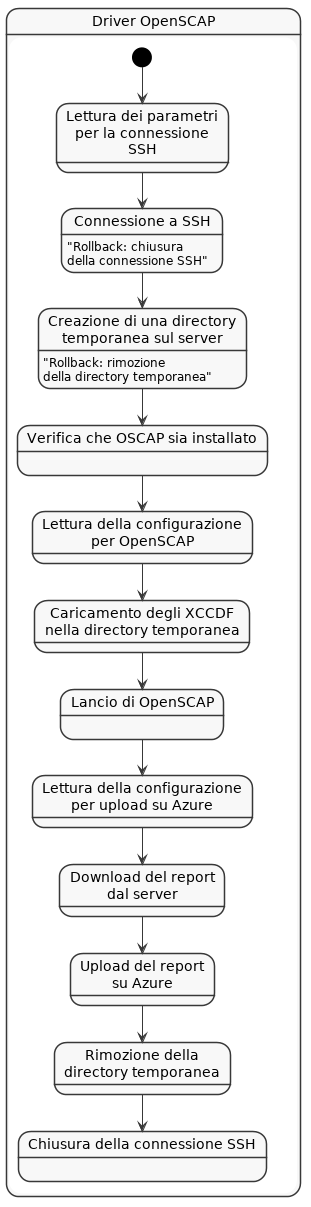
\includegraphics[height=15cm]{immagini/DRIVER_OPENSCAP.png}
\caption{Flusso di esecuzione del driver}\label{fig:flussodriver1}

\end{figure}

\subsubsection{Metadata}

\begin{js}
{
  "driver-name": "OpenSCAP_SSH",
  "description" : "",
  "schema" : {
        "read_ssh_configuration" : {
            "properties" : {
                "hostname" : {
                    "title" : "SSH Connection String",
                    "type" : "string",
                    "required": true
                },
                "username" : {
                    "title" : "Username",
                    "type" : "string",
                    "required": true
                },
                "password": {
                    "title":"Password",
                    "type":"password"
                },
                "private_key": {
                    "title": "SSH Private Key",
                    "type":"string",
                },
                "private_key_passphrase": {
                    "title":"Passphrase",
                    "type":"password"
                }
            },
            "title" : "Target",
            "type" : "object"
        },
        "read_xccdf_configuration":{
            "properties": {
                "xccdf": {
                    "title": "XCCDF",
                    "type": "string",
                    "required": true
                },
                "profile": {
                    "title": "Profile",
                    "type": "string",
                    "required":"true"
                },
                "fetch_remote_resources": {
                    "title": "Fetch remote resources declared in XCCDF",
                    "type": "boolean",
                    "default": false
                }
            },
            "title": "OpenSCAP settings",
            "type":"object"
        },
        "read_azure_configuration":{
            "properties": {
                "user": {
                    "title": "Username",
                    "type": "string",
                    "required": true
                },
                "access_key": {
                    "title": "Access Key",
                    "type": "password",
                    "required":true
                },
                "container_name": {
                    "title": "Azure Container name",
                    "type": "string",
                    "required":true
                }
            },
            "title": "Azure settings",
            "type":"object"
        }

    },
    "inputs": {
        "read_ssh_configuration": {
            "hostname": "string",
            "username": "string",
            "password": "password",
            "private_key": "string",
            "private_key_passphrase": "string"
        },
        "read_xccdf_configuration": {
            "xccdf": "string",
            "profile": "string",
            "fetch_remote_resources": "boolean"
        },
        "read_azure_configuration": {
            "user": "string",
            "access_key": "password",
            "container_name": "string"
        }
    },
    "outputs": {
        "report": "string"
    }
}
\end{js}
Il codice del driver è stato allegato nell'Appendice \ref{appendix:driver1}

\section{Controlli ad interazione umana}
Poiché, come già ampiamente trattato, non è possibile eseguire in maniera automatica tutti i controlli di sicurezza, l'obiettivo di questa tesi è
anche quello di fornire uno strumento per la verifica dei controlli di carattere procedurale che prevedono intrinsecamente un'interazione umana.

La modalità scelta è la somministrazione di questionari agli attori coinvolti nel controllo. A tal fine, una delle possibili strategie è quella di utilizzare
il linguaggio OCIL presente nel framework SCAP.

OCIL è un framework generico per la creazione di questionari ad interazione umana e non automatizzabili, definito nel documento NIST Interagency Report 7692 – Specification for the Open Checklist Interactive Language (OCIL) Version 2.0.
Le funzionalità di OCIL sono:
\begin{itemize}
    \item Possibilità di definire domande (con risposte di tipo booleano, scelta multipla, numerico, stringa)
    \item Possibilità di definire risposte predefinite per ciascuna domanda
    \item Possibilità di definire le azioni conseguenti alla risposta dell'utente 
    \item Possibilità di catalogare le risposte date
\end{itemize}
Un esempio di OCIL per la valutazione della \textit{FedRAMP readiness} è presente in appendice \ref{appendix:readiness}

\subsection{Driver Survey per Moon Cloud}

Si è voluto perciò integrare in Moon Cloud un driver ad interazione umana che, tramite un web-service, proponga all'utente un questionario e generi un report di feedback.
Nel caso di Moon Cloud, i questionari non sono descritti in OCIL ma utilizzando lo standard JSON Schema\footnote{JSON Schema \textit{http://www.json-schema.org/}}; è possibile eventualmente effettuare la traduzione mediante un foglio di trasformazione \textit{XSLT}.

Il test effettua il download della definizione del questionario da sottoporre, dopodiché lancia una web-application che offre il questionario all'utente. La web application è autenticata con nome utente e password, ed esposta tramite un reverse proxy dinamico chiamato \textit{traefik\footnote{Traefik: https://www.traefik.io}}.
\textit{Traefik} è un proxy per architetture a microservizi, in grado di leggere la lista dei container attivi dalle API Docker consentendo l'accesso ad eventuali servizi esposti sugli stessi.
I \textit{container} del driver \textit{Survey} vengono quindi  avviati con la \textit{label} \textit{"proxied"} e sono forniti tramite connessione SSL. Il certificato SSL viene automaticamente generato utilizzando il protocollo \textit{ACME}\footnote{ACME,  \textit{https://tools.ietf.org/html/draft-ietf-acme-acme-04}} e il servizio LetsEncrypt.

A questo punto viene inviata una notifica a mezzo \textit{e-mail} per il destinatario, con il link per accedere e compilare lo stesso.
Nel momento in cui il questionario viene sottomesso, viene generato un report in PDF, che è successivamente caricato in un \textit{Windows Azure Storage} analogamente al report \textit{OSCAP} precedentemente illustrato.

La difficoltà principale riscontrata nella realizzazione di questo driver risiede nell'introduzione di un processo manuale all'interno del framework Moon Cloud, pensato per eseguire test in modo automatico.
Il flusso di esecuzione, in questo caso, è invece caratterizzato da una fase bloccante che non termina finché l'utente non ha compilato il questionario stesso.
Lo \textit{scheduler} di Moon Cloud, per come originariamente ideato, programma l'esecuzione dei test eseguendone \textit{n} alla volta, dove \textit{n} è un parametro di concorrenza (\textit{--max-concurrency}) generalmente calcolato in base alla potenza computazionale e al numero di core disponibili sull'\textit{execution node}.

L'introduzione dell'azione bloccante ha perciò comportato una saturazione dei thread, rendendo impossibile lo \textit{scheduling} di nuovi test.
Questo problema è stato affrontato dapprima aumentando il valore di \textit{max-concurrency}, poi facendo scalare orizzontalmente il framework, tuttavia è necessaria una reingegnerizzazione del processo di esecuzione di alcune tipologie di test, etichettati come "bloccanti".

A tal fine sono state proposte due soluzioni:
\begin{itemize}
    \item La prima soluzione proposta è implementabile aggiungendo un \textit{timer} di durata massima all'esecuzione del test: quando il timer scade, il test viene rimosso restituendo un risultato \textit{False} e il container relativo viene cancellato.
\item La seconda soluzione proposta consiste nell'eseguire il driver in background, per poi monitorarne lo stato con un test ad esecuzione periodica. 
In questo caso avremmo quindi una evaluation rule così composta:
\begin{Verbatim}[frame=single]
a#1 implies a#2
\end{Verbatim}
In questo modo \textit{a\#1} lancia il driver "survey" in background terminando con "true", mentre \textit{a\#2} viene eseguito periodicamente per raccogliere il risultato del questionario, e restituisce "false" finché il questionario non è stato compilato.
\end{itemize}
\subsubsection{Flusso di esecuzione}
\begin{figure}[H]
\centering
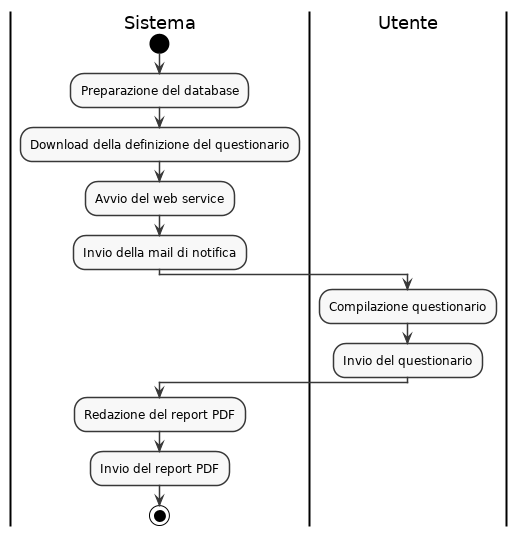
\includegraphics[height=15cm]{immagini/DRIVER_SURVEY.png}
\caption{Flusso di esecuzione del driver}\label{fig:flussodriver2}

\end{figure}
\subsubsection{Metadata}
\begin{js}
{
	"driver-name": "SurveyControl",
	"description": "",
	"schema": {
		"applicant": {
			"type": "object",
			"title": "Applicant Information",
			"properties": {
				"name": {
					"type": "string",
					"title": "Full Name"
				},
				"company": {
					"type": "string",
					"title": "Company"
				},
				"default_sender": {
					"type": "string",
					"title": "E-Mail address"
				}
			}
		},
        "survey_definition": {
            "type": "object",
            "title": "Survey definition",
            "properties": {
                "survey_url": {
                    "type": "string"
                    "title": "Survey definition URL"
                }
            }
        },
        "notification_email_settings": {
			"type": "object",
			"title": "SMTP Client Configuration",
			"properties": {
				"": {
					"type": "boolean",
					"title": "Use moon-cloud email service (it must be selected)",
					"default": true
				}
			}
		},
		"notification_email_subject": {
			"type": "object",
			"title": "Recipient Information",
			"properties": {
				"name": {
					"type": "string",
					"title": "Full Name"
				},
				"email": {
					"type": "string",
					"title": "E-Mail address"
				}
			}
		},
        "read_azure_configuration":{
            "properties": {
                "user": {
                    "title": "Username",
                    "type": "string",
                    "required": true
                },
                "access_key": {
                    "title": "Access Key",
                    "type": "password",
                    "required":true
                },
                "container_name": {
                    "title": "Azure Container name",
                    "type": "string",
                    "required":true
                }
            },
            "title": "Azure settings",
            "type":"object"
        }
	}
}


\end{js}
\end{document}
